\documentclass[twoside]{book}

% Packages required by doxygen
\usepackage{calc}
\usepackage{doxygen}
\usepackage{graphicx}
\usepackage[utf8]{inputenc}
\usepackage{makeidx}
\usepackage{multicol}
\usepackage{multirow}
\usepackage{fixltx2e}
\PassOptionsToPackage{warn}{textcomp}
\usepackage{textcomp}
\usepackage[nointegrals]{wasysym}
\usepackage[table]{xcolor}

% Font selection
\usepackage[T1]{fontenc}
\usepackage{mathptmx}
\usepackage[scaled=.90]{helvet}
\usepackage{courier}
\usepackage{amssymb}
\usepackage{sectsty}
\renewcommand{\familydefault}{\sfdefault}
\allsectionsfont{%
  \fontseries{bc}\selectfont%
  \color{darkgray}%
}
\renewcommand{\DoxyLabelFont}{%
  \fontseries{bc}\selectfont%
  \color{darkgray}%
}
\newcommand{\+}{\discretionary{\mbox{\scriptsize$\hookleftarrow$}}{}{}}

% Page & text layout
\usepackage{geometry}
\geometry{%
  a4paper,%
  top=2.5cm,%
  bottom=2.5cm,%
  left=2.5cm,%
  right=2.5cm%
}
\tolerance=750
\hfuzz=15pt
\hbadness=750
\setlength{\emergencystretch}{15pt}
\setlength{\parindent}{0cm}
\setlength{\parskip}{0.2cm}
\makeatletter
\renewcommand{\paragraph}{%
  \@startsection{paragraph}{4}{0ex}{-1.0ex}{1.0ex}{%
    \normalfont\normalsize\bfseries\SS@parafont%
  }%
}
\renewcommand{\subparagraph}{%
  \@startsection{subparagraph}{5}{0ex}{-1.0ex}{1.0ex}{%
    \normalfont\normalsize\bfseries\SS@subparafont%
  }%
}
\makeatother

% Headers & footers
\usepackage{fancyhdr}
\pagestyle{fancyplain}
\fancyhead[LE]{\fancyplain{}{\bfseries\thepage}}
\fancyhead[CE]{\fancyplain{}{}}
\fancyhead[RE]{\fancyplain{}{\bfseries\leftmark}}
\fancyhead[LO]{\fancyplain{}{\bfseries\rightmark}}
\fancyhead[CO]{\fancyplain{}{}}
\fancyhead[RO]{\fancyplain{}{\bfseries\thepage}}
\fancyfoot[LE]{\fancyplain{}{}}
\fancyfoot[CE]{\fancyplain{}{}}
\fancyfoot[RE]{\fancyplain{}{\bfseries\scriptsize Generated on Mon Aug 11 2014 01\+:01\+:55 for i\+Robot Roomba 500 Series S\+D\+K by Doxygen }}
\fancyfoot[LO]{\fancyplain{}{\bfseries\scriptsize Generated on Mon Aug 11 2014 01\+:01\+:55 for i\+Robot Roomba 500 Series S\+D\+K by Doxygen }}
\fancyfoot[CO]{\fancyplain{}{}}
\fancyfoot[RO]{\fancyplain{}{}}
\renewcommand{\footrulewidth}{0.4pt}
\renewcommand{\chaptermark}[1]{%
  \markboth{#1}{}%
}
\renewcommand{\sectionmark}[1]{%
  \markright{\thesection\ #1}%
}

% Indices & bibliography
\usepackage{natbib}
\usepackage[titles]{tocloft}
\setcounter{tocdepth}{3}
\setcounter{secnumdepth}{5}
\makeindex

% Hyperlinks (required, but should be loaded last)
\usepackage{ifpdf}
\ifpdf
  \usepackage[pdftex,pagebackref=true]{hyperref}
\else
  \usepackage[ps2pdf,pagebackref=true]{hyperref}
\fi
\hypersetup{%
  colorlinks=true,%
  linkcolor=blue,%
  citecolor=blue,%
  unicode%
}

% Custom commands
\newcommand{\clearemptydoublepage}{%
  \newpage{\pagestyle{empty}\cleardoublepage}%
}


%===== C O N T E N T S =====

\begin{document}

% Titlepage & ToC
\hypersetup{pageanchor=false,
             bookmarks=true,
             bookmarksnumbered=true,
             pdfencoding=unicode
            }
\pagenumbering{roman}
\begin{titlepage}
\vspace*{7cm}
\begin{center}%
{\Large i\+Robot Roomba 500 Series S\+D\+K \\[1ex]\large 1.\+0.\+0-\/alpha }\\
\vspace*{1cm}
{\large Generated by Doxygen 1.8.7}\\
\vspace*{0.5cm}
{\small Mon Aug 11 2014 01:01:55}\\
\end{center}
\end{titlepage}
\clearemptydoublepage
\tableofcontents
\clearemptydoublepage
\pagenumbering{arabic}
\hypersetup{pageanchor=true}

%--- Begin generated contents ---
\chapter{Hierarchical Index}
\section{Class Hierarchy}
This inheritance list is sorted roughly, but not completely, alphabetically\+:\begin{DoxyCompactList}
\item \contentsline{section}{roomba\+:\+:series500\+:\+:oi\+:\+:O\+I\+Encoder\+:\+:clock\+\_\+time\+\_\+t}{\pageref{structroomba_1_1series500_1_1oi_1_1_o_i_encoder_1_1clock__time__t}}{}
\item \contentsline{section}{roomba\+:\+:series500\+:\+:oi\+:\+:O\+I\+Encoder}{\pageref{classroomba_1_1series500_1_1oi_1_1_o_i_encoder}}{}
\begin{DoxyCompactList}
\item \contentsline{section}{O\+I\+Encoder\+\_\+\+T\+C}{\pageref{class_o_i_encoder___t_c}}{}
\end{DoxyCompactList}
\end{DoxyCompactList}

\chapter{Class Index}
\section{Class List}
Here are the classes, structs, unions and interfaces with brief descriptions\+:\begin{DoxyCompactList}
\item\contentsline{section}{\hyperlink{structroomba_1_1series500_1_1oi_1_1_o_i_encoder_1_1clock__time__t}{roomba\+::series500\+::oi\+::\+O\+I\+Encoder\+::clock\+\_\+time\+\_\+t} \\*Time representation for the scheduling methods }{\pageref{structroomba_1_1series500_1_1oi_1_1_o_i_encoder_1_1clock__time__t}}{}
\item\contentsline{section}{\hyperlink{classroomba_1_1series500_1_1oi_1_1_o_i_encoder}{roomba\+::series500\+::oi\+::\+O\+I\+Encoder} \\*The Roomba Open Interface (O\+I) \hyperlink{classroomba_1_1series500_1_1oi_1_1_o_i_encoder}{O\+I\+Encoder} static class }{\pageref{classroomba_1_1series500_1_1oi_1_1_o_i_encoder}}{}
\item\contentsline{section}{\hyperlink{class_o_i_encoder___t_c}{O\+I\+Encoder\+\_\+\+T\+C} }{\pageref{class_o_i_encoder___t_c}}{}
\end{DoxyCompactList}

\chapter{Class Documentation}
\hypertarget{classroomba_1_1series500_1_1_open_interface}{\section{roomba\+:\+:series500\+:\+:Open\+Interface Class Reference}
\label{classroomba_1_1series500_1_1_open_interface}\index{roomba\+::series500\+::\+Open\+Interface@{roomba\+::series500\+::\+Open\+Interface}}
}


The Roomba Open Interface (O\+I) class.  




{\ttfamily \#include $<$O\+I.\+h$>$}

Inheritance diagram for roomba\+:\+:series500\+:\+:Open\+Interface\+:\begin{figure}[H]
\begin{center}
\leavevmode
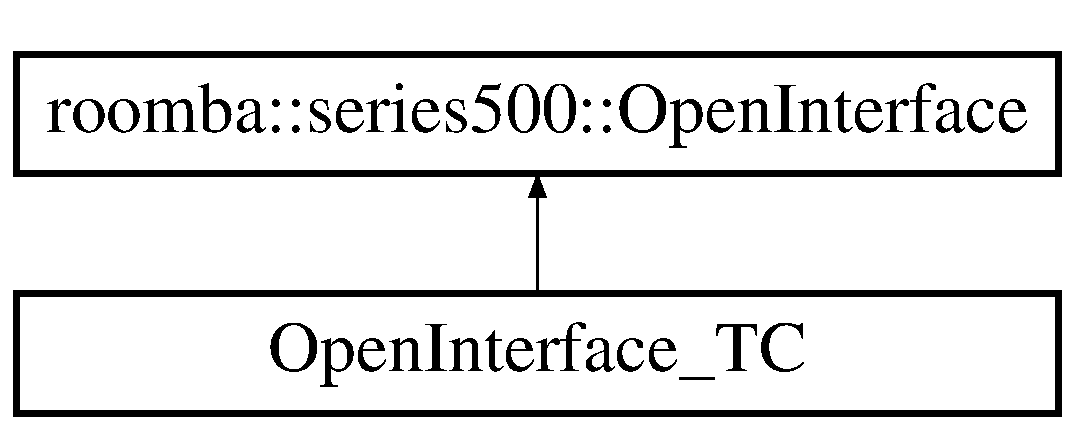
\includegraphics[height=2.000000cm]{classroomba_1_1series500_1_1_open_interface}
\end{center}
\end{figure}
\subsection*{Classes}
\begin{DoxyCompactItemize}
\item 
struct \hyperlink{structroomba_1_1series500_1_1_open_interface_1_1clock__time__t}{clock\+\_\+time\+\_\+t}
\begin{DoxyCompactList}\small\item\em Time representation for the scheduling methods. \end{DoxyCompactList}\end{DoxyCompactItemize}
\subsection*{Public Types}
\begin{DoxyCompactItemize}
\item 
\hypertarget{classroomba_1_1series500_1_1_open_interface_a43fc2ae1216e57cfb46901331b9ab4c7}{enum \hyperlink{classroomba_1_1series500_1_1_open_interface_a43fc2ae1216e57cfb46901331b9ab4c7}{Return\+Code} \+: int8\+\_\+t \{ \\*
{\bfseries S\+E\+R\+I\+A\+L\+\_\+\+T\+R\+A\+N\+S\+F\+E\+R\+\_\+\+F\+A\+I\+L\+U\+R\+E} = -\/100, 
{\bfseries I\+N\+V\+A\+L\+I\+D\+\_\+\+P\+A\+R\+A\+M\+E\+T\+E\+R} = -\/10, 
{\bfseries I\+N\+V\+A\+L\+I\+D\+\_\+\+M\+O\+D\+E\+\_\+\+F\+O\+R\+\_\+\+R\+E\+Q\+U\+E\+S\+T\+E\+D\+\_\+\+O\+P\+E\+R\+A\+T\+I\+O\+N} = -\/2, 
{\bfseries O\+I\+\_\+\+N\+O\+T\+\_\+\+S\+T\+A\+R\+T\+E\+D} = -\/1, 
\\*
{\bfseries S\+U\+C\+C\+E\+S\+S} = 0
 \}}\label{classroomba_1_1series500_1_1_open_interface_a43fc2ae1216e57cfb46901331b9ab4c7}

\begin{DoxyCompactList}\small\item\em Return codes. \end{DoxyCompactList}\item 
typedef struct \\*
\hyperlink{structroomba_1_1series500_1_1_open_interface_1_1clock__time__t}{roomba\+::series500\+::\+Open\+Interface\+::clock\+\_\+time\+\_\+t} \hyperlink{classroomba_1_1series500_1_1_open_interface_a28e1b87b0cce69349c416a7fcda3d624}{clock\+\_\+time\+\_\+t}
\begin{DoxyCompactList}\small\item\em Time representation for the scheduling methods. \end{DoxyCompactList}\end{DoxyCompactItemize}
\subsection*{Public Member Functions}
\begin{DoxyCompactItemize}
\item 
void \hyperlink{classroomba_1_1series500_1_1_open_interface_a3da6204e57a44fbd562fe5711126b069}{operator()} (const command\+::\+Op\+Code opcode\+\_\+, const std\+::vector$<$ uint8\+\_\+t $>$ \&data\+\_\+)
\begin{DoxyCompactList}\small\item\em Direct access to the Open Interface. \end{DoxyCompactList}\item 
void \hyperlink{classroomba_1_1series500_1_1_open_interface_a8ae1fddf62ac384a3956ee44fa4b51ee}{connect\+To\+Serial\+Bus} (const std\+::function$<$ size\+\_\+t(const uint8\+\_\+t $\ast$, size\+\_\+t)$>$ fn\+Serial\+Write\+\_\+)
\begin{DoxyCompactList}\small\item\em Establishes a serial channel with the hardware. \end{DoxyCompactList}\item 
void \hyperlink{classroomba_1_1series500_1_1_open_interface_a8a4ce79aebcc3a1c79ea66eb33dc0ec8}{end} (void) const 
\begin{DoxyCompactList}\small\item\em Releases control of the Roomba. \end{DoxyCompactList}\item 
\hyperlink{classroomba_1_1series500_1_1_open_interface_a43fc2ae1216e57cfb46901331b9ab4c7}{Return\+Code} \hyperlink{classroomba_1_1series500_1_1_open_interface_a5a0876c4910ead045cde79d49a99137a}{start} (void)
\begin{DoxyCompactList}\small\item\em Starts the O\+I. \end{DoxyCompactList}\item 
\hyperlink{classroomba_1_1series500_1_1_open_interface_a43fc2ae1216e57cfb46901331b9ab4c7}{Return\+Code} \hyperlink{classroomba_1_1series500_1_1_open_interface_a87e093214d5f7542062ac180d109f4fa}{baud} (const Baud\+Code baud\+\_\+code\+\_\+) const 
\begin{DoxyCompactList}\small\item\em Sets the baud rate in bits per second (bps). \end{DoxyCompactList}\item 
\hyperlink{classroomba_1_1series500_1_1_open_interface_a43fc2ae1216e57cfb46901331b9ab4c7}{Return\+Code} \hyperlink{classroomba_1_1series500_1_1_open_interface_a5bfb6443b97a05df2577a04856b46d13}{control} (void)
\begin{DoxyCompactList}\small\item\em The effect and usage of the Control command are identical to the Safe command. \end{DoxyCompactList}\item 
\hyperlink{classroomba_1_1series500_1_1_open_interface_a43fc2ae1216e57cfb46901331b9ab4c7}{Return\+Code} \hyperlink{classroomba_1_1series500_1_1_open_interface_a899d23ab053c49ac6555c27f2474b5a0}{safe} (void)
\begin{DoxyCompactList}\small\item\em Puts the O\+I into Safe mode. \end{DoxyCompactList}\item 
\hyperlink{classroomba_1_1series500_1_1_open_interface_a43fc2ae1216e57cfb46901331b9ab4c7}{Return\+Code} \hyperlink{classroomba_1_1series500_1_1_open_interface_acddf44604466bed9ffd120dcf22e59e7}{full} (void)
\begin{DoxyCompactList}\small\item\em Puts the O\+I into Full mode. \end{DoxyCompactList}\item 
\hyperlink{classroomba_1_1series500_1_1_open_interface_a43fc2ae1216e57cfb46901331b9ab4c7}{Return\+Code} \hyperlink{classroomba_1_1series500_1_1_open_interface_ab194541a8bf4475315f2385e5b04a697}{clean} (void)
\begin{DoxyCompactList}\small\item\em Starts the default cleaning mode. \end{DoxyCompactList}\item 
\hyperlink{classroomba_1_1series500_1_1_open_interface_a43fc2ae1216e57cfb46901331b9ab4c7}{Return\+Code} \hyperlink{classroomba_1_1series500_1_1_open_interface_a82020e146db624bbeeb47e613544876f}{max} (void)
\begin{DoxyCompactList}\small\item\em Starts the Max cleaning mode. \end{DoxyCompactList}\item 
\hyperlink{classroomba_1_1series500_1_1_open_interface_a43fc2ae1216e57cfb46901331b9ab4c7}{Return\+Code} \hyperlink{classroomba_1_1series500_1_1_open_interface_a7126b2aa105dea4b043c7acb4650f7c0}{spot} (void)
\begin{DoxyCompactList}\small\item\em Starts the Spot cleaning mode. \end{DoxyCompactList}\item 
\hyperlink{classroomba_1_1series500_1_1_open_interface_a43fc2ae1216e57cfb46901331b9ab4c7}{Return\+Code} \hyperlink{classroomba_1_1series500_1_1_open_interface_a45c9d9d77731030da42f9e3a337c45ed}{seek\+Dock} (void)
\begin{DoxyCompactList}\small\item\em Sends Roomba to the dock. \end{DoxyCompactList}\item 
\hyperlink{classroomba_1_1series500_1_1_open_interface_a43fc2ae1216e57cfb46901331b9ab4c7}{Return\+Code} \hyperlink{classroomba_1_1series500_1_1_open_interface_a9dcca64026dc1a9a563e90f0cfe97396}{schedule} (const bitmask\+::\+Days day\+\_\+mask\+\_\+, const \hyperlink{structroomba_1_1series500_1_1_open_interface_1_1clock__time__t}{clock\+\_\+time\+\_\+t} $\ast$const clock\+\_\+times\+\_\+) const 
\begin{DoxyCompactList}\small\item\em Sends Roomba a new schedule. \end{DoxyCompactList}\item 
\hyperlink{classroomba_1_1series500_1_1_open_interface_a43fc2ae1216e57cfb46901331b9ab4c7}{Return\+Code} \hyperlink{classroomba_1_1series500_1_1_open_interface_a68e09461fd2d7e3fbe20b1e70ea2a3a9}{set\+Day\+Time} (const Day day\+\_\+, const \hyperlink{structroomba_1_1series500_1_1_open_interface_1_1clock__time__t}{clock\+\_\+time\+\_\+t} clock\+\_\+time\+\_\+) const 
\begin{DoxyCompactList}\small\item\em Sets Roomba’s clock. \end{DoxyCompactList}\item 
\hyperlink{classroomba_1_1series500_1_1_open_interface_a43fc2ae1216e57cfb46901331b9ab4c7}{Return\+Code} \hyperlink{classroomba_1_1series500_1_1_open_interface_ae1abe0755730f35dd98d626c48d3f355}{power} (void)
\begin{DoxyCompactList}\small\item\em Powers down Roomba. \end{DoxyCompactList}\item 
\hyperlink{classroomba_1_1series500_1_1_open_interface_a43fc2ae1216e57cfb46901331b9ab4c7}{Return\+Code} \hyperlink{classroomba_1_1series500_1_1_open_interface_a0b02a89315ed3e6daa6b36b5f1327fc7}{drive} (const int16\+\_\+t velocity\+\_\+, const int16\+\_\+t radius\+\_\+) const 
\begin{DoxyCompactList}\small\item\em Controls Roomba’s drive wheels. \end{DoxyCompactList}\item 
\hyperlink{classroomba_1_1series500_1_1_open_interface_a43fc2ae1216e57cfb46901331b9ab4c7}{Return\+Code} \hyperlink{classroomba_1_1series500_1_1_open_interface_a3148367bdbf04abcb590c48adc03d2a1}{drive\+Direct} (const int16\+\_\+t right\+\_\+wheel\+\_\+velocity\+\_\+, const int16\+\_\+t left\+\_\+wheel\+\_\+velocity\+\_\+) const 
\begin{DoxyCompactList}\small\item\em Controls the forward and backward motion of Roomba’s drive wheels independently. \end{DoxyCompactList}\item 
\hyperlink{classroomba_1_1series500_1_1_open_interface_a43fc2ae1216e57cfb46901331b9ab4c7}{Return\+Code} \hyperlink{classroomba_1_1series500_1_1_open_interface_aec2dbec11bbd03d2b07403692d43a658}{drive\+P\+W\+M} (const int16\+\_\+t right\+\_\+wheel\+\_\+pwm\+\_\+, const int16\+\_\+t left\+\_\+wheel\+\_\+pwm\+\_\+) const 
\begin{DoxyCompactList}\small\item\em Controls the raw forward and backward motion of Roomba’s drive wheels independently. \end{DoxyCompactList}\item 
\hyperlink{classroomba_1_1series500_1_1_open_interface_a43fc2ae1216e57cfb46901331b9ab4c7}{Return\+Code} \hyperlink{classroomba_1_1series500_1_1_open_interface_a350b0236512caa59c8b887ad58e0ad95}{motors} (const bitmask\+::\+Motor\+States motor\+\_\+state\+\_\+mask\+\_\+) const 
\begin{DoxyCompactList}\small\item\em Controls the forward and backward motion of Roomba’s main brush, side brush, and vacuum independently. \end{DoxyCompactList}\item 
\hyperlink{classroomba_1_1series500_1_1_open_interface_a43fc2ae1216e57cfb46901331b9ab4c7}{Return\+Code} \hyperlink{classroomba_1_1series500_1_1_open_interface_ad5bfebf55b685a6c793bb948618bd265}{pwm\+Motors} (const int8\+\_\+t main\+\_\+brush\+\_\+, const int8\+\_\+t side\+\_\+brush\+\_\+, const int8\+\_\+t vacuum\+\_\+) const 
\begin{DoxyCompactList}\small\item\em Controls the speed of Roomba’s main brush, side brush, and vacuum independently. \end{DoxyCompactList}\item 
\hyperlink{classroomba_1_1series500_1_1_open_interface_a43fc2ae1216e57cfb46901331b9ab4c7}{Return\+Code} \hyperlink{classroomba_1_1series500_1_1_open_interface_a02b07148f3745190241059eca07bcad9}{leds} (const bitmask\+::display\+::\+L\+E\+Ds led\+\_\+mask\+\_\+, const uint8\+\_\+t color\+\_\+, const uint8\+\_\+t intensity\+\_\+) const 
\begin{DoxyCompactList}\small\item\em Controls the L\+E\+Ds. \end{DoxyCompactList}\item 
\hyperlink{classroomba_1_1series500_1_1_open_interface_a43fc2ae1216e57cfb46901331b9ab4c7}{Return\+Code} \hyperlink{classroomba_1_1series500_1_1_open_interface_a9d7f8c1cca2d76a71fae39d7b29ebe94}{scheduling\+L\+E\+Ds} (const bitmask\+::\+Days day\+\_\+mask\+\_\+, const bitmask\+::display\+::\+Scheduling\+L\+E\+Ds led\+\_\+mask\+\_\+) const 
\begin{DoxyCompactList}\small\item\em Controls the state of the scheduling L\+E\+Ds present on the Roomba 560 and 570. \end{DoxyCompactList}\item 
\hyperlink{classroomba_1_1series500_1_1_open_interface_a43fc2ae1216e57cfb46901331b9ab4c7}{Return\+Code} \hyperlink{classroomba_1_1series500_1_1_open_interface_a76c9b0291da94519b91ec5e6d9409838}{digit\+L\+E\+Ds\+Raw} (const bitmask\+::display\+::\+Digit\+N raw\+\_\+leds\+\_\+\mbox{[}4\mbox{]}) const 
\begin{DoxyCompactList}\small\item\em Controls the 7 segment displays. \end{DoxyCompactList}\item 
\hyperlink{classroomba_1_1series500_1_1_open_interface_a43fc2ae1216e57cfb46901331b9ab4c7}{Return\+Code} \hyperlink{classroomba_1_1series500_1_1_open_interface_a60f023e5d923f0cd66a5f69e0b094c8a}{digit\+L\+E\+Ds\+A\+S\+C\+I\+I} (const char ascii\+\_\+leds\+\_\+\mbox{[}4\mbox{]}) const 
\begin{DoxyCompactList}\small\item\em Controls the 7 segment displays using A\+S\+C\+I\+I character codes. \end{DoxyCompactList}\item 
\hyperlink{classroomba_1_1series500_1_1_open_interface_a43fc2ae1216e57cfb46901331b9ab4c7}{Return\+Code} \hyperlink{classroomba_1_1series500_1_1_open_interface_a4e44856c9785a94f84b74d87138db7ec}{buttons} (const bitmask\+::\+Buttons button\+\_\+mask\+\_\+) const 
\begin{DoxyCompactList}\small\item\em Push Roomba’s buttons. \end{DoxyCompactList}\item 
\hyperlink{classroomba_1_1series500_1_1_open_interface_a43fc2ae1216e57cfb46901331b9ab4c7}{Return\+Code} \hyperlink{classroomba_1_1series500_1_1_open_interface_a316b270bdf96b6b89c9ecc8a4f7a39bd}{song} (const uint8\+\_\+t song\+\_\+number\+\_\+, const std\+::vector$<$ std\+::pair$<$ Note, uint8\+\_\+t $>$ $>$ \&notes\+\_\+) const 
\begin{DoxyCompactList}\small\item\em Specify songs to be played at a later time. \end{DoxyCompactList}\item 
\hyperlink{classroomba_1_1series500_1_1_open_interface_a43fc2ae1216e57cfb46901331b9ab4c7}{Return\+Code} \hyperlink{classroomba_1_1series500_1_1_open_interface_a89c1c582ee1254d283fdb3ebbeb6ba67}{play} (const uint8\+\_\+t song\+\_\+number\+\_\+) const 
\begin{DoxyCompactList}\small\item\em Select a song to play. \end{DoxyCompactList}\item 
\hyperlink{classroomba_1_1series500_1_1_open_interface_a43fc2ae1216e57cfb46901331b9ab4c7}{Return\+Code} \hyperlink{classroomba_1_1series500_1_1_open_interface_af7b042d7919548d8feae666f097e3392}{sensors} (const sensor\+::\+Packet\+Id packet\+\_\+id\+\_\+) const 
\begin{DoxyCompactList}\small\item\em Request sensor data. \end{DoxyCompactList}\item 
\hyperlink{classroomba_1_1series500_1_1_open_interface_a43fc2ae1216e57cfb46901331b9ab4c7}{Return\+Code} \hyperlink{classroomba_1_1series500_1_1_open_interface_a1a1f69be99bb2833580bddcaa60bf15a}{query\+List} (const std\+::vector$<$ sensor\+::\+Packet\+Id $>$ \&packet\+\_\+ids\+\_\+) const 
\begin{DoxyCompactList}\small\item\em Request list of sensor packets. \end{DoxyCompactList}\item 
\hyperlink{classroomba_1_1series500_1_1_open_interface_a43fc2ae1216e57cfb46901331b9ab4c7}{Return\+Code} \hyperlink{classroomba_1_1series500_1_1_open_interface_a902485dee6502c9f89627ae824c5b1d1}{stream} (const std\+::vector$<$ sensor\+::\+Packet\+Id $>$ \&packet\+\_\+ids\+\_\+) const 
\begin{DoxyCompactList}\small\item\em Start a data stream based on a query list. \end{DoxyCompactList}\item 
\hyperlink{classroomba_1_1series500_1_1_open_interface_a43fc2ae1216e57cfb46901331b9ab4c7}{Return\+Code} \hyperlink{classroomba_1_1series500_1_1_open_interface_a610783954ac02c9a6ee349e864143554}{pause\+Resume\+Stream} (void) const 
\begin{DoxyCompactList}\small\item\em Stop and restart the stream. \end{DoxyCompactList}\end{DoxyCompactItemize}
\subsection*{Protected Attributes}
\begin{DoxyCompactItemize}
\item 
\hypertarget{classroomba_1_1series500_1_1_open_interface_adc93297613591cfdb94229ac1da0befd}{std\+::function$<$ size\+\_\+t(const \\*
uint8\+\_\+t $\ast$, size\+\_\+t)$>$ {\bfseries \+\_\+fn\+Serial\+Write}}\label{classroomba_1_1series500_1_1_open_interface_adc93297613591cfdb94229ac1da0befd}

\item 
\hypertarget{classroomba_1_1series500_1_1_open_interface_a2491dd5d1efe4358d7d5b76e272163c3}{O\+I\+Mode {\bfseries \+\_\+mode}}\label{classroomba_1_1series500_1_1_open_interface_a2491dd5d1efe4358d7d5b76e272163c3}

\end{DoxyCompactItemize}


\subsection{Detailed Description}
The Roomba Open Interface (O\+I) class. 

The Roomba Open Interface (O\+I) is a software interface for controlling and manipulating Roomba’s behavior. The software interface lets you manipulate Roomba’s behavior and read its sensors through a series of commands, including mode commands, actuator commands, song commands, and sensor commands that you send to the Roomba’s serial port by way of a P\+C or microcontroller that is connected to the Mini-\/\+D\+I\+N connector. 

\subsection{Member Typedef Documentation}
\hypertarget{classroomba_1_1series500_1_1_open_interface_a28e1b87b0cce69349c416a7fcda3d624}{\index{roomba\+::series500\+::\+Open\+Interface@{roomba\+::series500\+::\+Open\+Interface}!clock\+\_\+time\+\_\+t@{clock\+\_\+time\+\_\+t}}
\index{clock\+\_\+time\+\_\+t@{clock\+\_\+time\+\_\+t}!roomba\+::series500\+::\+Open\+Interface@{roomba\+::series500\+::\+Open\+Interface}}
\subsubsection[{clock\+\_\+time\+\_\+t}]{\setlength{\rightskip}{0pt plus 5cm}typedef struct {\bf roomba\+::series500\+::\+Open\+Interface\+::clock\+\_\+time\+\_\+t}  {\bf roomba\+::series500\+::\+Open\+Interface\+::clock\+\_\+time\+\_\+t}}}\label{classroomba_1_1series500_1_1_open_interface_a28e1b87b0cce69349c416a7fcda3d624}


Time representation for the scheduling methods. 

This struct represents time in military time with the two fields hour and minute. The values in the structure are initialized to zero upon instantiation. 

\subsection{Member Function Documentation}
\hypertarget{classroomba_1_1series500_1_1_open_interface_a87e093214d5f7542062ac180d109f4fa}{\index{roomba\+::series500\+::\+Open\+Interface@{roomba\+::series500\+::\+Open\+Interface}!baud@{baud}}
\index{baud@{baud}!roomba\+::series500\+::\+Open\+Interface@{roomba\+::series500\+::\+Open\+Interface}}
\subsubsection[{baud}]{\setlength{\rightskip}{0pt plus 5cm}{\bf Open\+Interface\+::\+Return\+Code} roomba\+::series500\+::\+Open\+Interface\+::baud (
\begin{DoxyParamCaption}
\item[{const Baud\+Code}]{baud\+\_\+code\+\_\+}
\end{DoxyParamCaption}
) const}}\label{classroomba_1_1series500_1_1_open_interface_a87e093214d5f7542062ac180d109f4fa}


Sets the baud rate in bits per second (bps). 

This command sets the baud rate in bits per second (bps) at which O\+I commands and data are sent according to the baud code sent in the data byte. 
\begin{DoxyParams}[1]{Parameters}
\mbox{\tt in}  & {\em baud\+\_\+code} & \\
\hline
\end{DoxyParams}
\begin{DoxyNote}{Note}
The default baud rate at power up is 115200 bps. 

Available in modes\+: Passive, Safe, or Full. 
\end{DoxyNote}

\begin{DoxyRetVals}{Return values}
{\em S\+U\+C\+C\+E\+S\+S} & \\
\hline
{\em O\+I\+\_\+\+N\+O\+T\+\_\+\+S\+T\+A\+R\+T\+E\+D} & \\
\hline
{\em S\+E\+R\+I\+A\+L\+\_\+\+T\+R\+A\+N\+S\+F\+E\+R\+\_\+\+F\+A\+I\+L\+U\+R\+E} & \\
\hline
\end{DoxyRetVals}
\hypertarget{classroomba_1_1series500_1_1_open_interface_a4e44856c9785a94f84b74d87138db7ec}{\index{roomba\+::series500\+::\+Open\+Interface@{roomba\+::series500\+::\+Open\+Interface}!buttons@{buttons}}
\index{buttons@{buttons}!roomba\+::series500\+::\+Open\+Interface@{roomba\+::series500\+::\+Open\+Interface}}
\subsubsection[{buttons}]{\setlength{\rightskip}{0pt plus 5cm}{\bf Return\+Code} roomba\+::series500\+::\+Open\+Interface\+::buttons (
\begin{DoxyParamCaption}
\item[{const bitmask\+::\+Buttons}]{button\+\_\+mask\+\_\+}
\end{DoxyParamCaption}
) const}}\label{classroomba_1_1series500_1_1_open_interface_a4e44856c9785a94f84b74d87138db7ec}


Push Roomba’s buttons. 

This command lets you push Roomba’s buttons. The buttons will automatically release after 1/6th of a second. 
\begin{DoxyParams}[1]{Parameters}
\mbox{\tt in}  & {\em button\+\_\+mask} & \\
\hline
\end{DoxyParams}
\begin{DoxyNote}{Note}
Available in modes\+: Passive, Safe, or Full. 
\end{DoxyNote}
\hypertarget{classroomba_1_1series500_1_1_open_interface_ab194541a8bf4475315f2385e5b04a697}{\index{roomba\+::series500\+::\+Open\+Interface@{roomba\+::series500\+::\+Open\+Interface}!clean@{clean}}
\index{clean@{clean}!roomba\+::series500\+::\+Open\+Interface@{roomba\+::series500\+::\+Open\+Interface}}
\subsubsection[{clean}]{\setlength{\rightskip}{0pt plus 5cm}{\bf Open\+Interface\+::\+Return\+Code} roomba\+::series500\+::\+Open\+Interface\+::clean (
\begin{DoxyParamCaption}
\item[{void}]{}
\end{DoxyParamCaption}
)}}\label{classroomba_1_1series500_1_1_open_interface_ab194541a8bf4475315f2385e5b04a697}


Starts the default cleaning mode. 

\begin{DoxyNote}{Note}
Available in modes\+: Passive, Safe, or Full. 

Changes mode to\+: Passive. 
\end{DoxyNote}

\begin{DoxyRetVals}{Return values}
{\em S\+U\+C\+C\+E\+S\+S} & \\
\hline
{\em O\+I\+\_\+\+N\+O\+T\+\_\+\+S\+T\+A\+R\+T\+E\+D} & \\
\hline
{\em S\+E\+R\+I\+A\+L\+\_\+\+T\+R\+A\+N\+S\+F\+E\+R\+\_\+\+F\+A\+I\+L\+U\+R\+E} & \\
\hline
\end{DoxyRetVals}
\hypertarget{classroomba_1_1series500_1_1_open_interface_a8ae1fddf62ac384a3956ee44fa4b51ee}{\index{roomba\+::series500\+::\+Open\+Interface@{roomba\+::series500\+::\+Open\+Interface}!connect\+To\+Serial\+Bus@{connect\+To\+Serial\+Bus}}
\index{connect\+To\+Serial\+Bus@{connect\+To\+Serial\+Bus}!roomba\+::series500\+::\+Open\+Interface@{roomba\+::series500\+::\+Open\+Interface}}
\subsubsection[{connect\+To\+Serial\+Bus}]{\setlength{\rightskip}{0pt plus 5cm}void roomba\+::series500\+::\+Open\+Interface\+::connect\+To\+Serial\+Bus (
\begin{DoxyParamCaption}
\item[{const std\+::function$<$ size\+\_\+t(const uint8\+\_\+t $\ast$, size\+\_\+t)$>$}]{fn\+Serial\+Write\+\_\+}
\end{DoxyParamCaption}
)}}\label{classroomba_1_1series500_1_1_open_interface_a8ae1fddf62ac384a3956ee44fa4b51ee}


Establishes a serial channel with the hardware. 

This method must be called before any other methods of this class. It establishes a serial channel between the Open Interface class and the underlying hardware. The default baud for communicating with the Roomba outside the Open Interface is 115200, if the external microcontroller is unable to communicate at that speed, an alternative baud, 19200, is available. To enable the slower baud on the Roomba you must power-\/on the Roomba by holding down the clean/power button, or the Roomba can be signaled on the baud rate change line. 
\begin{DoxyParams}[1]{Parameters}
\mbox{\tt in}  & {\em fn\+Serial\+Write} & A function that writes to the serial bus at either 115200 or 19200 baud. \\
\hline
\end{DoxyParams}
\begin{DoxyWarning}{Warning}
If the baud rate of fn\+Serial\+Write is not synchronized to the baud rate of the Roomba, then this class will be unable to communicate with the Roomba's Open Interface. 
\end{DoxyWarning}
\hypertarget{classroomba_1_1series500_1_1_open_interface_a5bfb6443b97a05df2577a04856b46d13}{\index{roomba\+::series500\+::\+Open\+Interface@{roomba\+::series500\+::\+Open\+Interface}!control@{control}}
\index{control@{control}!roomba\+::series500\+::\+Open\+Interface@{roomba\+::series500\+::\+Open\+Interface}}
\subsubsection[{control}]{\setlength{\rightskip}{0pt plus 5cm}{\bf Open\+Interface\+::\+Return\+Code} roomba\+::series500\+::\+Open\+Interface\+::control (
\begin{DoxyParamCaption}
\item[{void}]{}
\end{DoxyParamCaption}
)}}\label{classroomba_1_1series500_1_1_open_interface_a5bfb6443b97a05df2577a04856b46d13}


The effect and usage of the Control command are identical to the Safe command. 

\begin{DoxySeeAlso}{See also}
\hyperlink{classroomba_1_1series500_1_1_open_interface_a899d23ab053c49ac6555c27f2474b5a0}{Open\+Interface\+::safe} 
\end{DoxySeeAlso}
\hypertarget{classroomba_1_1series500_1_1_open_interface_a60f023e5d923f0cd66a5f69e0b094c8a}{\index{roomba\+::series500\+::\+Open\+Interface@{roomba\+::series500\+::\+Open\+Interface}!digit\+L\+E\+Ds\+A\+S\+C\+I\+I@{digit\+L\+E\+Ds\+A\+S\+C\+I\+I}}
\index{digit\+L\+E\+Ds\+A\+S\+C\+I\+I@{digit\+L\+E\+Ds\+A\+S\+C\+I\+I}!roomba\+::series500\+::\+Open\+Interface@{roomba\+::series500\+::\+Open\+Interface}}
\subsubsection[{digit\+L\+E\+Ds\+A\+S\+C\+I\+I}]{\setlength{\rightskip}{0pt plus 5cm}{\bf Return\+Code} roomba\+::series500\+::\+Open\+Interface\+::digit\+L\+E\+Ds\+A\+S\+C\+I\+I (
\begin{DoxyParamCaption}
\item[{const char}]{ascii\+\_\+leds\+\_\+\mbox{[}4\mbox{]}}
\end{DoxyParamCaption}
) const}}\label{classroomba_1_1series500_1_1_open_interface_a60f023e5d923f0cd66a5f69e0b094c8a}


Controls the 7 segment displays using A\+S\+C\+I\+I character codes. 

This command controls the four 7 segment displays on the Roomba 560 and 570 using A\+S\+C\+I\+I character codes. Because a 7 segment display is not sufficient to display alphabetic characters properly, all characters are an approximation 
\begin{DoxyParams}[1]{Parameters}
\mbox{\tt in}  & {\em ascii\+\_\+leds} & An A\+S\+C\+I\+I char array (valid values range from (32-\/126). \\
\hline
\end{DoxyParams}
\begin{DoxyNote}{Note}
Available in modes\+: Safe or Full 
\end{DoxyNote}
\begin{DoxyWarning}{Warning}
Not all A\+S\+C\+I\+I codes are implemented. 
\end{DoxyWarning}
\hypertarget{classroomba_1_1series500_1_1_open_interface_a76c9b0291da94519b91ec5e6d9409838}{\index{roomba\+::series500\+::\+Open\+Interface@{roomba\+::series500\+::\+Open\+Interface}!digit\+L\+E\+Ds\+Raw@{digit\+L\+E\+Ds\+Raw}}
\index{digit\+L\+E\+Ds\+Raw@{digit\+L\+E\+Ds\+Raw}!roomba\+::series500\+::\+Open\+Interface@{roomba\+::series500\+::\+Open\+Interface}}
\subsubsection[{digit\+L\+E\+Ds\+Raw}]{\setlength{\rightskip}{0pt plus 5cm}{\bf Return\+Code} roomba\+::series500\+::\+Open\+Interface\+::digit\+L\+E\+Ds\+Raw (
\begin{DoxyParamCaption}
\item[{const bitmask\+::display\+::\+Digit\+N}]{raw\+\_\+leds\+\_\+\mbox{[}4\mbox{]}}
\end{DoxyParamCaption}
) const}}\label{classroomba_1_1series500_1_1_open_interface_a76c9b0291da94519b91ec5e6d9409838}


Controls the 7 segment displays. 

This command controls the four 7 segment displays on the Roomba 560 and 570. 
\begin{DoxyParams}[1]{Parameters}
\mbox{\tt in}  & {\em raw\+\_\+leds} & An array representing the four 7 segment display values. \\
\hline
\end{DoxyParams}
\begin{DoxyNote}{Note}
All use red L\+E\+Ds 

Available in modes\+: Safe or Full. 
\end{DoxyNote}
\hypertarget{classroomba_1_1series500_1_1_open_interface_a0b02a89315ed3e6daa6b36b5f1327fc7}{\index{roomba\+::series500\+::\+Open\+Interface@{roomba\+::series500\+::\+Open\+Interface}!drive@{drive}}
\index{drive@{drive}!roomba\+::series500\+::\+Open\+Interface@{roomba\+::series500\+::\+Open\+Interface}}
\subsubsection[{drive}]{\setlength{\rightskip}{0pt plus 5cm}{\bf Return\+Code} roomba\+::series500\+::\+Open\+Interface\+::drive (
\begin{DoxyParamCaption}
\item[{const int16\+\_\+t}]{velocity\+\_\+, }
\item[{const int16\+\_\+t}]{radius\+\_\+}
\end{DoxyParamCaption}
) const}}\label{classroomba_1_1series500_1_1_open_interface_a0b02a89315ed3e6daa6b36b5f1327fc7}


Controls Roomba’s drive wheels. 

This command controls Roomba’s drive wheels. A Drive command with a positive velocity and a positive radius makes Roomba drive forward while turning toward the left. A negative radius makes Roomba turn toward the right. Special cases for the radius make Roomba turn in place or drive straight, as specified below. A negative velocity makes Roomba drive backward. 
\begin{DoxyParams}[1]{Parameters}
\mbox{\tt in}  & {\em velocity} & (-\/500 – 500) The average velocity of the drive wheels in millimeters per second (mm/s). \\
\hline
\mbox{\tt in}  & {\em radius} & (-\/2000 – 2000) The radius in millimeters at which Roomba will turn. The radius is measured from the center of the turning circle to the center of Roomba. \\
\hline
\end{DoxyParams}
\begin{DoxyParagraph}{Special cases}

\end{DoxyParagraph}
\begin{DoxyParagraph}{}
Straight = 32768 (0x8000) or 32767 (0x7\+F\+F\+F) 
\end{DoxyParagraph}
\begin{DoxyParagraph}{}
Turn in place clockwise = -\/1 
\end{DoxyParagraph}
\begin{DoxyParagraph}{}
Turn in place counter-\/clockwise = 1 
\end{DoxyParagraph}
\begin{DoxyNote}{Note}
Available in modes\+: Safe or Full. 
\end{DoxyNote}
\begin{DoxyWarning}{Warning}
Internal and environmental restrictions may prevent Roomba from accurately carrying out some drive commands. 
\end{DoxyWarning}
\hypertarget{classroomba_1_1series500_1_1_open_interface_a3148367bdbf04abcb590c48adc03d2a1}{\index{roomba\+::series500\+::\+Open\+Interface@{roomba\+::series500\+::\+Open\+Interface}!drive\+Direct@{drive\+Direct}}
\index{drive\+Direct@{drive\+Direct}!roomba\+::series500\+::\+Open\+Interface@{roomba\+::series500\+::\+Open\+Interface}}
\subsubsection[{drive\+Direct}]{\setlength{\rightskip}{0pt plus 5cm}{\bf Return\+Code} roomba\+::series500\+::\+Open\+Interface\+::drive\+Direct (
\begin{DoxyParamCaption}
\item[{const int16\+\_\+t}]{right\+\_\+wheel\+\_\+velocity\+\_\+, }
\item[{const int16\+\_\+t}]{left\+\_\+wheel\+\_\+velocity\+\_\+}
\end{DoxyParamCaption}
) const}}\label{classroomba_1_1series500_1_1_open_interface_a3148367bdbf04abcb590c48adc03d2a1}


Controls the forward and backward motion of Roomba’s drive wheels independently. 

This command lets you control the forward and backward motion of Roomba’s drive wheels independently. A positive velocity makes that wheel drive forward, while a negative velocity makes it drive backward. 
\begin{DoxyParams}[1]{Parameters}
\mbox{\tt in}  & {\em right\+\_\+wheel\+\_\+velocity} & (-\/500 – 500) The velocity of the right wheel in millimeters per second (mm/s). \\
\hline
\mbox{\tt in}  & {\em left\+\_\+wheel\+\_\+velocity} & (-\/500 – 500) The velocity of the left wheel in millimeters per second (mm/s). \\
\hline
\end{DoxyParams}
\begin{DoxyNote}{Note}
Available in modes\+: Safe or Full. 
\end{DoxyNote}
\hypertarget{classroomba_1_1series500_1_1_open_interface_aec2dbec11bbd03d2b07403692d43a658}{\index{roomba\+::series500\+::\+Open\+Interface@{roomba\+::series500\+::\+Open\+Interface}!drive\+P\+W\+M@{drive\+P\+W\+M}}
\index{drive\+P\+W\+M@{drive\+P\+W\+M}!roomba\+::series500\+::\+Open\+Interface@{roomba\+::series500\+::\+Open\+Interface}}
\subsubsection[{drive\+P\+W\+M}]{\setlength{\rightskip}{0pt plus 5cm}{\bf Return\+Code} roomba\+::series500\+::\+Open\+Interface\+::drive\+P\+W\+M (
\begin{DoxyParamCaption}
\item[{const int16\+\_\+t}]{right\+\_\+wheel\+\_\+pwm\+\_\+, }
\item[{const int16\+\_\+t}]{left\+\_\+wheel\+\_\+pwm\+\_\+}
\end{DoxyParamCaption}
) const}}\label{classroomba_1_1series500_1_1_open_interface_aec2dbec11bbd03d2b07403692d43a658}


Controls the raw forward and backward motion of Roomba’s drive wheels independently. 

This command lets you control the raw forward and backward motion of Roomba’s drive wheels independently. A positive P\+W\+M makes that wheel drive forward, while a negative P\+W\+M makes it drive backward. 
\begin{DoxyParams}[1]{Parameters}
\mbox{\tt in}  & {\em right\+\_\+wheel\+\_\+pwm} & (-\/255 – 255) The P\+W\+M of the right wheel. \\
\hline
\mbox{\tt in}  & {\em left\+\_\+wheel\+\_\+pwm} & (-\/255 – 255) The P\+W\+M of the left wheel. \\
\hline
\end{DoxyParams}
\begin{DoxyNote}{Note}
Available in modes\+: Safe or Full. 
\end{DoxyNote}
\hypertarget{classroomba_1_1series500_1_1_open_interface_a8a4ce79aebcc3a1c79ea66eb33dc0ec8}{\index{roomba\+::series500\+::\+Open\+Interface@{roomba\+::series500\+::\+Open\+Interface}!end@{end}}
\index{end@{end}!roomba\+::series500\+::\+Open\+Interface@{roomba\+::series500\+::\+Open\+Interface}}
\subsubsection[{end}]{\setlength{\rightskip}{0pt plus 5cm}void roomba\+::series500\+::\+Open\+Interface\+::end (
\begin{DoxyParamCaption}
\item[{void}]{}
\end{DoxyParamCaption}
) const}}\label{classroomba_1_1series500_1_1_open_interface_a8a4ce79aebcc3a1c79ea66eb33dc0ec8}


Releases control of the Roomba. 

This method with set the O\+I Mode to passive and return the Roomba to its docking station. It will also reinitialize the class member variables to restore it to a clean state. \hypertarget{classroomba_1_1series500_1_1_open_interface_acddf44604466bed9ffd120dcf22e59e7}{\index{roomba\+::series500\+::\+Open\+Interface@{roomba\+::series500\+::\+Open\+Interface}!full@{full}}
\index{full@{full}!roomba\+::series500\+::\+Open\+Interface@{roomba\+::series500\+::\+Open\+Interface}}
\subsubsection[{full}]{\setlength{\rightskip}{0pt plus 5cm}{\bf Open\+Interface\+::\+Return\+Code} roomba\+::series500\+::\+Open\+Interface\+::full (
\begin{DoxyParamCaption}
\item[{void}]{}
\end{DoxyParamCaption}
)}}\label{classroomba_1_1series500_1_1_open_interface_acddf44604466bed9ffd120dcf22e59e7}


Puts the O\+I into Full mode. 

This command gives you complete control over Roomba by putting the O\+I into Full mode, and turning off the cliff, wheel-\/drop and internal charger safety features. \begin{DoxyNote}{Note}
Available in modes\+: Passive, Safe, or Full. 

Changes mode to\+: Full. 
\end{DoxyNote}

\begin{DoxyRetVals}{Return values}
{\em S\+U\+C\+C\+E\+S\+S} & \\
\hline
{\em O\+I\+\_\+\+N\+O\+T\+\_\+\+S\+T\+A\+R\+T\+E\+D} & \\
\hline
{\em S\+E\+R\+I\+A\+L\+\_\+\+T\+R\+A\+N\+S\+F\+E\+R\+\_\+\+F\+A\+I\+L\+U\+R\+E} & \\
\hline
\end{DoxyRetVals}
\hypertarget{classroomba_1_1series500_1_1_open_interface_a02b07148f3745190241059eca07bcad9}{\index{roomba\+::series500\+::\+Open\+Interface@{roomba\+::series500\+::\+Open\+Interface}!leds@{leds}}
\index{leds@{leds}!roomba\+::series500\+::\+Open\+Interface@{roomba\+::series500\+::\+Open\+Interface}}
\subsubsection[{leds}]{\setlength{\rightskip}{0pt plus 5cm}{\bf Return\+Code} roomba\+::series500\+::\+Open\+Interface\+::leds (
\begin{DoxyParamCaption}
\item[{const bitmask\+::display\+::\+L\+E\+Ds}]{led\+\_\+mask\+\_\+, }
\item[{const uint8\+\_\+t}]{color\+\_\+, }
\item[{const uint8\+\_\+t}]{intensity\+\_\+}
\end{DoxyParamCaption}
) const}}\label{classroomba_1_1series500_1_1_open_interface_a02b07148f3745190241059eca07bcad9}


Controls the L\+E\+Ds. 

This command controls the L\+E\+Ds common to all models of Roomba 500. Clean/\+Power uses a bicolor (red/green) L\+E\+D. The intensity and color of this L\+E\+D can be controlled with 8-\/bit resolution. 
\begin{DoxyParams}[1]{Parameters}
\mbox{\tt in}  & {\em led\+\_\+mask} & \\
\hline
\mbox{\tt in}  & {\em color} & 0 = green, 255 = red. Intermediate values are intermediate colors (orange, yellow, etc). \\
\hline
\mbox{\tt in}  & {\em intensity} & 0 = off, 255 = full intensity. Intermediate values are intermediate intensities. \\
\hline
\end{DoxyParams}
\begin{DoxyNote}{Note}
Home and Spot use green L\+E\+Ds\+: 0 = off, 1 = on. 

Check Robot uses an orange L\+E\+D. 

Debris uses a blue L\+E\+D. 

Available in modes\+: Safe or Full. 
\end{DoxyNote}
\hypertarget{classroomba_1_1series500_1_1_open_interface_a82020e146db624bbeeb47e613544876f}{\index{roomba\+::series500\+::\+Open\+Interface@{roomba\+::series500\+::\+Open\+Interface}!max@{max}}
\index{max@{max}!roomba\+::series500\+::\+Open\+Interface@{roomba\+::series500\+::\+Open\+Interface}}
\subsubsection[{max}]{\setlength{\rightskip}{0pt plus 5cm}{\bf Open\+Interface\+::\+Return\+Code} roomba\+::series500\+::\+Open\+Interface\+::max (
\begin{DoxyParamCaption}
\item[{void}]{}
\end{DoxyParamCaption}
)}}\label{classroomba_1_1series500_1_1_open_interface_a82020e146db624bbeeb47e613544876f}


Starts the Max cleaning mode. 

\begin{DoxyNote}{Note}
Available in modes\+: Passive, Safe, or Full. 

Changes mode to\+: Passive. 
\end{DoxyNote}

\begin{DoxyRetVals}{Return values}
{\em S\+U\+C\+C\+E\+S\+S} & \\
\hline
{\em O\+I\+\_\+\+N\+O\+T\+\_\+\+S\+T\+A\+R\+T\+E\+D} & \\
\hline
{\em S\+E\+R\+I\+A\+L\+\_\+\+T\+R\+A\+N\+S\+F\+E\+R\+\_\+\+F\+A\+I\+L\+U\+R\+E} & \\
\hline
\end{DoxyRetVals}
\hypertarget{classroomba_1_1series500_1_1_open_interface_a350b0236512caa59c8b887ad58e0ad95}{\index{roomba\+::series500\+::\+Open\+Interface@{roomba\+::series500\+::\+Open\+Interface}!motors@{motors}}
\index{motors@{motors}!roomba\+::series500\+::\+Open\+Interface@{roomba\+::series500\+::\+Open\+Interface}}
\subsubsection[{motors}]{\setlength{\rightskip}{0pt plus 5cm}{\bf Return\+Code} roomba\+::series500\+::\+Open\+Interface\+::motors (
\begin{DoxyParamCaption}
\item[{const bitmask\+::\+Motor\+States}]{motor\+\_\+state\+\_\+mask\+\_\+}
\end{DoxyParamCaption}
) const}}\label{classroomba_1_1series500_1_1_open_interface_a350b0236512caa59c8b887ad58e0ad95}


Controls the forward and backward motion of Roomba’s main brush, side brush, and vacuum independently. 

This command lets you control the forward and backward motion of Roomba’s main brush, side brush, and vacuum independently. Motor velocity cannot be controlled with this command, all motors will run at maximum speed when enabled. The main brush and side brush can be run in either direction. The vacuum only runs forward. 
\begin{DoxyParams}[1]{Parameters}
\mbox{\tt in}  & {\em motor\+\_\+state\+\_\+mask} & \\
\hline
\end{DoxyParams}
\begin{DoxyNote}{Note}
Available in modes\+: Safe or Full. 
\end{DoxyNote}
\hypertarget{classroomba_1_1series500_1_1_open_interface_a3da6204e57a44fbd562fe5711126b069}{\index{roomba\+::series500\+::\+Open\+Interface@{roomba\+::series500\+::\+Open\+Interface}!operator()@{operator()}}
\index{operator()@{operator()}!roomba\+::series500\+::\+Open\+Interface@{roomba\+::series500\+::\+Open\+Interface}}
\subsubsection[{operator()}]{\setlength{\rightskip}{0pt plus 5cm}void roomba\+::series500\+::\+Open\+Interface\+::operator() (
\begin{DoxyParamCaption}
\item[{const command\+::\+Op\+Code}]{opcode\+\_\+, }
\item[{const std\+::vector$<$ uint8\+\_\+t $>$ \&}]{data\+\_\+}
\end{DoxyParamCaption}
)}}\label{classroomba_1_1series500_1_1_open_interface_a3da6204e57a44fbd562fe5711126b069}


Direct access to the Open Interface. 

Direct access sends bytes directly to the Open Interface. Direct access is potentially dangerous, because the parameters are not checked and the device can be left in a \char`\"{}waiting\char`\"{} state. 
\begin{DoxyParams}[1]{Parameters}
\mbox{\tt in}  & {\em opcode} & \\
\hline
\mbox{\tt in}  & {\em \mbox{[}data\mbox{]}} & An optional list of parameters for the Op\+Code specified. \\
\hline
\end{DoxyParams}
\begin{DoxyWarning}{Warning}
Use of direct access will invalidate the current state of the object, and will incur the overhead associated with polling the state of the device to restore the current state. 
\end{DoxyWarning}
\hypertarget{classroomba_1_1series500_1_1_open_interface_a610783954ac02c9a6ee349e864143554}{\index{roomba\+::series500\+::\+Open\+Interface@{roomba\+::series500\+::\+Open\+Interface}!pause\+Resume\+Stream@{pause\+Resume\+Stream}}
\index{pause\+Resume\+Stream@{pause\+Resume\+Stream}!roomba\+::series500\+::\+Open\+Interface@{roomba\+::series500\+::\+Open\+Interface}}
\subsubsection[{pause\+Resume\+Stream}]{\setlength{\rightskip}{0pt plus 5cm}{\bf Return\+Code} roomba\+::series500\+::\+Open\+Interface\+::pause\+Resume\+Stream (
\begin{DoxyParamCaption}
\item[{void}]{}
\end{DoxyParamCaption}
) const}}\label{classroomba_1_1series500_1_1_open_interface_a610783954ac02c9a6ee349e864143554}


Stop and restart the stream. 

This command lets you stop and restart the steam without clearing the list of requested packets. \begin{DoxyNote}{Note}
Available in modes\+: Passive, Safe, or Full. 
\end{DoxyNote}
\hypertarget{classroomba_1_1series500_1_1_open_interface_a89c1c582ee1254d283fdb3ebbeb6ba67}{\index{roomba\+::series500\+::\+Open\+Interface@{roomba\+::series500\+::\+Open\+Interface}!play@{play}}
\index{play@{play}!roomba\+::series500\+::\+Open\+Interface@{roomba\+::series500\+::\+Open\+Interface}}
\subsubsection[{play}]{\setlength{\rightskip}{0pt plus 5cm}{\bf Return\+Code} roomba\+::series500\+::\+Open\+Interface\+::play (
\begin{DoxyParamCaption}
\item[{const uint8\+\_\+t}]{song\+\_\+number\+\_\+}
\end{DoxyParamCaption}
) const}}\label{classroomba_1_1series500_1_1_open_interface_a89c1c582ee1254d283fdb3ebbeb6ba67}


Select a song to play. 

This command lets you select a song to play from the songs added to Roomba using the Song command. You must add one or more songs to Roomba using the Song command in order for the Play command to work. 
\begin{DoxyParams}[1]{Parameters}
\mbox{\tt in}  & {\em song\+\_\+number} & (0-\/4) The number of the song Roomba is to play. \\
\hline
\end{DoxyParams}
\begin{DoxyNote}{Note}
Available in modes\+: Safe or Full 
\end{DoxyNote}
\begin{DoxySeeAlso}{See also}
\hyperlink{classroomba_1_1series500_1_1_open_interface_a316b270bdf96b6b89c9ecc8a4f7a39bd}{Open\+Interface\+::song} 
\end{DoxySeeAlso}
\hypertarget{classroomba_1_1series500_1_1_open_interface_ae1abe0755730f35dd98d626c48d3f355}{\index{roomba\+::series500\+::\+Open\+Interface@{roomba\+::series500\+::\+Open\+Interface}!power@{power}}
\index{power@{power}!roomba\+::series500\+::\+Open\+Interface@{roomba\+::series500\+::\+Open\+Interface}}
\subsubsection[{power}]{\setlength{\rightskip}{0pt plus 5cm}{\bf Open\+Interface\+::\+Return\+Code} roomba\+::series500\+::\+Open\+Interface\+::power (
\begin{DoxyParamCaption}
\item[{void}]{}
\end{DoxyParamCaption}
)}}\label{classroomba_1_1series500_1_1_open_interface_ae1abe0755730f35dd98d626c48d3f355}


Powers down Roomba. 

This command powers down Roomba. The O\+I can be in Passive, Safe, or Full mode to accept this command. \begin{DoxyNote}{Note}
Available in modes\+: Passive, Safe, or Full. 

Changes mode to\+: Passive. 
\end{DoxyNote}
\hypertarget{classroomba_1_1series500_1_1_open_interface_ad5bfebf55b685a6c793bb948618bd265}{\index{roomba\+::series500\+::\+Open\+Interface@{roomba\+::series500\+::\+Open\+Interface}!pwm\+Motors@{pwm\+Motors}}
\index{pwm\+Motors@{pwm\+Motors}!roomba\+::series500\+::\+Open\+Interface@{roomba\+::series500\+::\+Open\+Interface}}
\subsubsection[{pwm\+Motors}]{\setlength{\rightskip}{0pt plus 5cm}{\bf Return\+Code} roomba\+::series500\+::\+Open\+Interface\+::pwm\+Motors (
\begin{DoxyParamCaption}
\item[{const int8\+\_\+t}]{main\+\_\+brush\+\_\+, }
\item[{const int8\+\_\+t}]{side\+\_\+brush\+\_\+, }
\item[{const int8\+\_\+t}]{vacuum\+\_\+}
\end{DoxyParamCaption}
) const}}\label{classroomba_1_1series500_1_1_open_interface_ad5bfebf55b685a6c793bb948618bd265}


Controls the speed of Roomba’s main brush, side brush, and vacuum independently. 

This command lets you control the speed of Roomba’s main brush, side brush, and vacuum independently. With each parameter, you specify the duty cycle for the low side driver (max 127). Positive speeds turn the motor in its default (cleaning) direction. For example, if you want to control a motor with 25\% of battery voltage, choose a duty cycle of 127 $\ast$ 25\% $\sim$ 32. 
\begin{DoxyParams}[1]{Parameters}
\mbox{\tt in}  & {\em main\+\_\+brush} & (-\/127 – 127) \\
\hline
\mbox{\tt in}  & {\em side\+\_\+brush} & (-\/127 – 127) \\
\hline
\mbox{\tt in}  & {\em vacuum} & (0 – 127) \\
\hline
\end{DoxyParams}
\begin{DoxyNote}{Note}
The vacuum only runs forward. 

The main brush and side brush can be run in either direction. 

Default direction for the side brush is counter-\/clockwise. 

Default direction for the main brush/flapper is inward. 

Available in modes\+: Safe or Full. 
\end{DoxyNote}
\hypertarget{classroomba_1_1series500_1_1_open_interface_a1a1f69be99bb2833580bddcaa60bf15a}{\index{roomba\+::series500\+::\+Open\+Interface@{roomba\+::series500\+::\+Open\+Interface}!query\+List@{query\+List}}
\index{query\+List@{query\+List}!roomba\+::series500\+::\+Open\+Interface@{roomba\+::series500\+::\+Open\+Interface}}
\subsubsection[{query\+List}]{\setlength{\rightskip}{0pt plus 5cm}{\bf Return\+Code} roomba\+::series500\+::\+Open\+Interface\+::query\+List (
\begin{DoxyParamCaption}
\item[{const std\+::vector$<$ sensor\+::\+Packet\+Id $>$ \&}]{packet\+\_\+ids\+\_\+}
\end{DoxyParamCaption}
) const}}\label{classroomba_1_1series500_1_1_open_interface_a1a1f69be99bb2833580bddcaa60bf15a}


Request list of sensor packets. 

This command lets you ask for a list of sensor packets. The result is returned once, as in the Sensors command. The robot returns the packets in the order you specify. 
\begin{DoxyParams}{Parameters}
{\em packet\+\_\+ids} & A vector of packet ids \\
\hline
\end{DoxyParams}
\begin{DoxyNote}{Note}
Available in modes\+: Passive, Safe, or Full. 
\end{DoxyNote}
\hypertarget{classroomba_1_1series500_1_1_open_interface_a899d23ab053c49ac6555c27f2474b5a0}{\index{roomba\+::series500\+::\+Open\+Interface@{roomba\+::series500\+::\+Open\+Interface}!safe@{safe}}
\index{safe@{safe}!roomba\+::series500\+::\+Open\+Interface@{roomba\+::series500\+::\+Open\+Interface}}
\subsubsection[{safe}]{\setlength{\rightskip}{0pt plus 5cm}{\bf Open\+Interface\+::\+Return\+Code} roomba\+::series500\+::\+Open\+Interface\+::safe (
\begin{DoxyParamCaption}
\item[{void}]{}
\end{DoxyParamCaption}
)}}\label{classroomba_1_1series500_1_1_open_interface_a899d23ab053c49ac6555c27f2474b5a0}


Puts the O\+I into Safe mode. 

This command puts the O\+I into Safe mode, enabling user control of Roomba. It turns off all L\+E\+Ds. The O\+I can be in Passive, Safe, or Full mode to accept this command. \begin{DoxyNote}{Note}
If a safety condition occurs (see above) Roomba reverts automatically to Passive mode. 

Available in modes\+: Passive, Safe, or Full. 

Changes mode to\+: Safe. 
\end{DoxyNote}

\begin{DoxyRetVals}{Return values}
{\em S\+U\+C\+C\+E\+S\+S} & \\
\hline
{\em O\+I\+\_\+\+N\+O\+T\+\_\+\+S\+T\+A\+R\+T\+E\+D} & \\
\hline
{\em S\+E\+R\+I\+A\+L\+\_\+\+T\+R\+A\+N\+S\+F\+E\+R\+\_\+\+F\+A\+I\+L\+U\+R\+E} & \\
\hline
\end{DoxyRetVals}
\hypertarget{classroomba_1_1series500_1_1_open_interface_a9dcca64026dc1a9a563e90f0cfe97396}{\index{roomba\+::series500\+::\+Open\+Interface@{roomba\+::series500\+::\+Open\+Interface}!schedule@{schedule}}
\index{schedule@{schedule}!roomba\+::series500\+::\+Open\+Interface@{roomba\+::series500\+::\+Open\+Interface}}
\subsubsection[{schedule}]{\setlength{\rightskip}{0pt plus 5cm}{\bf Open\+Interface\+::\+Return\+Code} roomba\+::series500\+::\+Open\+Interface\+::schedule (
\begin{DoxyParamCaption}
\item[{const bitmask\+::\+Days}]{day\+\_\+mask\+\_\+, }
\item[{const {\bf clock\+\_\+time\+\_\+t} $\ast$const}]{clock\+\_\+times\+\_\+}
\end{DoxyParamCaption}
) const}}\label{classroomba_1_1series500_1_1_open_interface_a9dcca64026dc1a9a563e90f0cfe97396}


Sends Roomba a new schedule. 

This command sends Roomba a new schedule. To disable scheduled cleaning, send all 0s. 
\begin{DoxyParams}[1]{Parameters}
\mbox{\tt in}  & {\em day\+\_\+mask} & A bitmask representing the days of the week \\
\hline
\mbox{\tt in}  & {\em clock\+\_\+times\+\_\+} & A sparse array of \hyperlink{structroomba_1_1series500_1_1_open_interface_1_1clock__time__t}{clock\+\_\+time\+\_\+t} variables following \{ Sun time, Mon time, ..., Sat time \}. \\
\hline
\end{DoxyParams}
\begin{DoxyNote}{Note}
The day\+\_\+mask variable will determine which days the array elements will be applied to, disabled days will be zero filled. 

If a \hyperlink{structroomba_1_1series500_1_1_open_interface_1_1clock__time__t}{clock\+\_\+time\+\_\+t} variable contains any values out of range, then the corresponding day will be ignored. 

If Roomba’s schedule or clock button is pressed, this command will be ignored. 

Available in modes\+: Passive, Safe, or Full. 
\end{DoxyNote}

\begin{DoxyRetVals}{Return values}
{\em S\+U\+C\+C\+E\+S\+S} & \\
\hline
{\em O\+I\+\_\+\+N\+O\+T\+\_\+\+S\+T\+A\+R\+T\+E\+D} & \\
\hline
{\em S\+E\+R\+I\+A\+L\+\_\+\+T\+R\+A\+N\+S\+F\+E\+R\+\_\+\+F\+A\+I\+L\+U\+R\+E} & \\
\hline
\end{DoxyRetVals}
\hypertarget{classroomba_1_1series500_1_1_open_interface_a9d7f8c1cca2d76a71fae39d7b29ebe94}{\index{roomba\+::series500\+::\+Open\+Interface@{roomba\+::series500\+::\+Open\+Interface}!scheduling\+L\+E\+Ds@{scheduling\+L\+E\+Ds}}
\index{scheduling\+L\+E\+Ds@{scheduling\+L\+E\+Ds}!roomba\+::series500\+::\+Open\+Interface@{roomba\+::series500\+::\+Open\+Interface}}
\subsubsection[{scheduling\+L\+E\+Ds}]{\setlength{\rightskip}{0pt plus 5cm}{\bf Return\+Code} roomba\+::series500\+::\+Open\+Interface\+::scheduling\+L\+E\+Ds (
\begin{DoxyParamCaption}
\item[{const bitmask\+::\+Days}]{day\+\_\+mask\+\_\+, }
\item[{const bitmask\+::display\+::\+Scheduling\+L\+E\+Ds}]{led\+\_\+mask\+\_\+}
\end{DoxyParamCaption}
) const}}\label{classroomba_1_1series500_1_1_open_interface_a9d7f8c1cca2d76a71fae39d7b29ebe94}


Controls the state of the scheduling L\+E\+Ds present on the Roomba 560 and 570. 


\begin{DoxyParams}[1]{Parameters}
\mbox{\tt in}  & {\em day\+\_\+mask} & \\
\hline
\mbox{\tt in}  & {\em led\+\_\+mask} & \\
\hline
\end{DoxyParams}
\begin{DoxyNote}{Note}
All use red L\+E\+Ds 

Available in modes\+: Safe or Full. 
\end{DoxyNote}
\hypertarget{classroomba_1_1series500_1_1_open_interface_a45c9d9d77731030da42f9e3a337c45ed}{\index{roomba\+::series500\+::\+Open\+Interface@{roomba\+::series500\+::\+Open\+Interface}!seek\+Dock@{seek\+Dock}}
\index{seek\+Dock@{seek\+Dock}!roomba\+::series500\+::\+Open\+Interface@{roomba\+::series500\+::\+Open\+Interface}}
\subsubsection[{seek\+Dock}]{\setlength{\rightskip}{0pt plus 5cm}{\bf Open\+Interface\+::\+Return\+Code} roomba\+::series500\+::\+Open\+Interface\+::seek\+Dock (
\begin{DoxyParamCaption}
\item[{void}]{}
\end{DoxyParamCaption}
)}}\label{classroomba_1_1series500_1_1_open_interface_a45c9d9d77731030da42f9e3a337c45ed}


Sends Roomba to the dock. 

\begin{DoxyNote}{Note}
Available in modes\+: Passive, Safe, or Full. 

Changes mode to\+: Passive. 
\end{DoxyNote}

\begin{DoxyRetVals}{Return values}
{\em S\+U\+C\+C\+E\+S\+S} & \\
\hline
{\em O\+I\+\_\+\+N\+O\+T\+\_\+\+S\+T\+A\+R\+T\+E\+D} & \\
\hline
{\em S\+E\+R\+I\+A\+L\+\_\+\+T\+R\+A\+N\+S\+F\+E\+R\+\_\+\+F\+A\+I\+L\+U\+R\+E} & \\
\hline
\end{DoxyRetVals}
\hypertarget{classroomba_1_1series500_1_1_open_interface_af7b042d7919548d8feae666f097e3392}{\index{roomba\+::series500\+::\+Open\+Interface@{roomba\+::series500\+::\+Open\+Interface}!sensors@{sensors}}
\index{sensors@{sensors}!roomba\+::series500\+::\+Open\+Interface@{roomba\+::series500\+::\+Open\+Interface}}
\subsubsection[{sensors}]{\setlength{\rightskip}{0pt plus 5cm}{\bf Return\+Code} roomba\+::series500\+::\+Open\+Interface\+::sensors (
\begin{DoxyParamCaption}
\item[{const sensor\+::\+Packet\+Id}]{packet\+\_\+id\+\_\+}
\end{DoxyParamCaption}
) const}}\label{classroomba_1_1series500_1_1_open_interface_af7b042d7919548d8feae666f097e3392}


Request sensor data. 

This command requests the O\+I to send a packet of sensor data bytes. There are 58 different sensor data packets. Each provides a value of a specific sensor or group of sensors. 
\begin{DoxyParams}[1]{Parameters}
\mbox{\tt in}  & {\em packet\+\_\+id} & Identifies which of the 58 sensor data packets should be sent back by the O\+I. \\
\hline
\end{DoxyParams}
\begin{DoxyNote}{Note}
A value of 100 indicates a packet with all of the sensor data. Values of 0 through 6 and 101 through 107 indicate specific subgroups of the sensor data. 

Available in modes\+: Passive, Safe, or Full. 
\end{DoxyNote}
\hypertarget{classroomba_1_1series500_1_1_open_interface_a68e09461fd2d7e3fbe20b1e70ea2a3a9}{\index{roomba\+::series500\+::\+Open\+Interface@{roomba\+::series500\+::\+Open\+Interface}!set\+Day\+Time@{set\+Day\+Time}}
\index{set\+Day\+Time@{set\+Day\+Time}!roomba\+::series500\+::\+Open\+Interface@{roomba\+::series500\+::\+Open\+Interface}}
\subsubsection[{set\+Day\+Time}]{\setlength{\rightskip}{0pt plus 5cm}{\bf Open\+Interface\+::\+Return\+Code} roomba\+::series500\+::\+Open\+Interface\+::set\+Day\+Time (
\begin{DoxyParamCaption}
\item[{const Day}]{day\+\_\+, }
\item[{const {\bf clock\+\_\+time\+\_\+t}}]{clock\+\_\+time\+\_\+}
\end{DoxyParamCaption}
) const}}\label{classroomba_1_1series500_1_1_open_interface_a68e09461fd2d7e3fbe20b1e70ea2a3a9}


Sets Roomba’s clock. 


\begin{DoxyParams}[1]{Parameters}
\mbox{\tt in}  & {\em day} & \\
\hline
\mbox{\tt in}  & {\em clock} & time (hour \mbox{[}0-\/23\mbox{]} and minute \mbox{[}0-\/59\mbox{]}) \\
\hline
\end{DoxyParams}
\begin{DoxyNote}{Note}
If Roomba’s schedule or clock button is pressed, this command will be ignored. 

Available in modes\+: Passive, Safe, or Full. 
\end{DoxyNote}

\begin{DoxyRetVals}{Return values}
{\em S\+U\+C\+C\+E\+S\+S} & \\
\hline
{\em O\+I\+\_\+\+N\+O\+T\+\_\+\+S\+T\+A\+R\+T\+E\+D} & \\
\hline
{\em I\+N\+V\+A\+L\+I\+D\+\_\+\+P\+A\+R\+A\+M\+E\+T\+E\+R} & \\
\hline
{\em S\+E\+R\+I\+A\+L\+\_\+\+T\+R\+A\+N\+S\+F\+E\+R\+\_\+\+F\+A\+I\+L\+U\+R\+E} & \\
\hline
\end{DoxyRetVals}
\hypertarget{classroomba_1_1series500_1_1_open_interface_a316b270bdf96b6b89c9ecc8a4f7a39bd}{\index{roomba\+::series500\+::\+Open\+Interface@{roomba\+::series500\+::\+Open\+Interface}!song@{song}}
\index{song@{song}!roomba\+::series500\+::\+Open\+Interface@{roomba\+::series500\+::\+Open\+Interface}}
\subsubsection[{song}]{\setlength{\rightskip}{0pt plus 5cm}{\bf Return\+Code} roomba\+::series500\+::\+Open\+Interface\+::song (
\begin{DoxyParamCaption}
\item[{const uint8\+\_\+t}]{song\+\_\+number\+\_\+, }
\item[{const std\+::vector$<$ std\+::pair$<$ Note, uint8\+\_\+t $>$ $>$ \&}]{notes\+\_\+}
\end{DoxyParamCaption}
) const}}\label{classroomba_1_1series500_1_1_open_interface_a316b270bdf96b6b89c9ecc8a4f7a39bd}


Specify songs to be played at a later time. 

This command lets you specify up to four songs to the O\+I that you can play at a later time. Each song is associated with a song number. The Play command uses the song number to identify your song selection. Each song can contain up to sixteen notes. Each note is associated with a note number that uses M\+I\+D\+I note definitions and a duration that is specified in increments of 1/64th of a second. 
\begin{DoxyParams}[1]{Parameters}
\mbox{\tt in}  & {\em song\+\_\+number} & (0-\/4) The song number associated with the specific song. \\
\hline
\mbox{\tt in}  & {\em song} & A vector of std\+::pairs composed of Note and duration. \\
\hline
\end{DoxyParams}
\begin{DoxyNote}{Note}
If you send a second Song command, using the same song number, the old song is overwritten. 

Available in modes\+: Passive, Safe, or Full. 
\end{DoxyNote}
\begin{DoxySeeAlso}{See also}
\hyperlink{classroomba_1_1series500_1_1_open_interface_a89c1c582ee1254d283fdb3ebbeb6ba67}{Open\+Interface\+::play} 
\end{DoxySeeAlso}
\hypertarget{classroomba_1_1series500_1_1_open_interface_a7126b2aa105dea4b043c7acb4650f7c0}{\index{roomba\+::series500\+::\+Open\+Interface@{roomba\+::series500\+::\+Open\+Interface}!spot@{spot}}
\index{spot@{spot}!roomba\+::series500\+::\+Open\+Interface@{roomba\+::series500\+::\+Open\+Interface}}
\subsubsection[{spot}]{\setlength{\rightskip}{0pt plus 5cm}{\bf Open\+Interface\+::\+Return\+Code} roomba\+::series500\+::\+Open\+Interface\+::spot (
\begin{DoxyParamCaption}
\item[{void}]{}
\end{DoxyParamCaption}
)}}\label{classroomba_1_1series500_1_1_open_interface_a7126b2aa105dea4b043c7acb4650f7c0}


Starts the Spot cleaning mode. 

\begin{DoxyNote}{Note}
Available in modes\+: Passive, Safe, or Full. 

Changes mode to\+: Passive. 
\end{DoxyNote}

\begin{DoxyRetVals}{Return values}
{\em S\+U\+C\+C\+E\+S\+S} & \\
\hline
{\em O\+I\+\_\+\+N\+O\+T\+\_\+\+S\+T\+A\+R\+T\+E\+D} & \\
\hline
{\em S\+E\+R\+I\+A\+L\+\_\+\+T\+R\+A\+N\+S\+F\+E\+R\+\_\+\+F\+A\+I\+L\+U\+R\+E} & \\
\hline
\end{DoxyRetVals}
\hypertarget{classroomba_1_1series500_1_1_open_interface_a5a0876c4910ead045cde79d49a99137a}{\index{roomba\+::series500\+::\+Open\+Interface@{roomba\+::series500\+::\+Open\+Interface}!start@{start}}
\index{start@{start}!roomba\+::series500\+::\+Open\+Interface@{roomba\+::series500\+::\+Open\+Interface}}
\subsubsection[{start}]{\setlength{\rightskip}{0pt plus 5cm}{\bf Open\+Interface\+::\+Return\+Code} roomba\+::series500\+::\+Open\+Interface\+::start (
\begin{DoxyParamCaption}
\item[{void}]{}
\end{DoxyParamCaption}
)}}\label{classroomba_1_1series500_1_1_open_interface_a5a0876c4910ead045cde79d49a99137a}


Starts the O\+I. 

You must always send the Start command before sending any other commands to the O\+I. \begin{DoxyNote}{Note}
Available in modes\+: Passive, Safe, or Full. 

Changes mode to\+: Passive. Roomba beeps once to acknowledge it is starting from “off” mode. 
\end{DoxyNote}

\begin{DoxyRetVals}{Return values}
{\em S\+U\+C\+C\+E\+S\+S} & \\
\hline
{\em S\+E\+R\+I\+A\+L\+\_\+\+T\+R\+A\+N\+S\+F\+E\+R\+\_\+\+F\+A\+I\+L\+U\+R\+E} & \\
\hline
\end{DoxyRetVals}
\hypertarget{classroomba_1_1series500_1_1_open_interface_a902485dee6502c9f89627ae824c5b1d1}{\index{roomba\+::series500\+::\+Open\+Interface@{roomba\+::series500\+::\+Open\+Interface}!stream@{stream}}
\index{stream@{stream}!roomba\+::series500\+::\+Open\+Interface@{roomba\+::series500\+::\+Open\+Interface}}
\subsubsection[{stream}]{\setlength{\rightskip}{0pt plus 5cm}{\bf Return\+Code} roomba\+::series500\+::\+Open\+Interface\+::stream (
\begin{DoxyParamCaption}
\item[{const std\+::vector$<$ sensor\+::\+Packet\+Id $>$ \&}]{packet\+\_\+ids\+\_\+}
\end{DoxyParamCaption}
) const}}\label{classroomba_1_1series500_1_1_open_interface_a902485dee6502c9f89627ae824c5b1d1}


Start a data stream based on a query list. 

This command starts a stream of data packets. The list of packets requested is sent every 15 ms, which is the rate Roomba uses to update data. 
\begin{DoxyParams}{Parameters}
{\em } & note This method of requesting sensor data is best if you are controlling Roomba over a wireless network (which has poor real-\/time characteristics) with software running on a desktop computer. \\
\hline
\end{DoxyParams}
\begin{DoxyNote}{Note}
Available in modes\+: Passive, Safe, or Full. 
\end{DoxyNote}


The documentation for this class was generated from the following files\+:\begin{DoxyCompactItemize}
\item 
/\+Users/zachary\+\_\+fields/\+Development/bitbucket/irobot-\/roomba-\/500-\/series-\/sdk/O\+I.\+h\item 
/\+Users/zachary\+\_\+fields/\+Development/bitbucket/irobot-\/roomba-\/500-\/series-\/sdk/O\+I.\+cpp\end{DoxyCompactItemize}

\hypertarget{class_open_interface___t_c}{\section{Open\+Interface\+\_\+\+T\+C Class Reference}
\label{class_open_interface___t_c}\index{Open\+Interface\+\_\+\+T\+C@{Open\+Interface\+\_\+\+T\+C}}
}
Inheritance diagram for Open\+Interface\+\_\+\+T\+C\+:\begin{figure}[H]
\begin{center}
\leavevmode
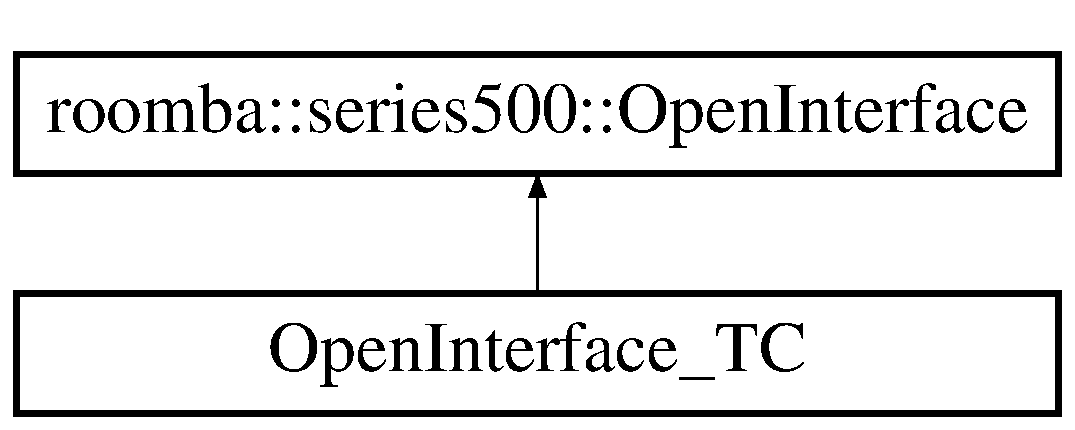
\includegraphics[height=2.000000cm]{class_open_interface___t_c}
\end{center}
\end{figure}
\subsection*{Additional Inherited Members}


The documentation for this class was generated from the following file\+:\begin{DoxyCompactItemize}
\item 
/\+Users/zachary\+\_\+fields/\+Development/bitbucket/irobot-\/roomba-\/500-\/series-\/sdk/gtest/gtest\+\_\+\+O\+I.\+cpp\end{DoxyCompactItemize}

%--- End generated contents ---

% Index
\newpage
\phantomsection
\addcontentsline{toc}{chapter}{Index}
\printindex

\end{document}
